\newchapt{Performance Evaluation}{chapt8}{Performance Evaluation}


%%%%%%%%%%%%%%%%%%%%%%%%%%%%%%%%
%%%%%%   Experimental Results%%%
%%%%%%%%%%%%%%%%%%%%%%%%%%%%%%%%
\section{Experimental Results}
\label{sec:IR_OUT}

The results of the extrusion and tapered structures computation,
together with keyslice image vectorization, are stored in the 2D
image coordinate system. To generate the final 3D model, these
data need to be transformed back into the 3D world coordinate system.
Let $P(x,y)$ be a point in the 2D image coordinate system, and let $P'(x,y,z)$
be the 3D world coordinate of $P$, where $y$ is the depth coordinate.
For all points in the same contour, the points lie in the same plane and
hence have the same value of $y$.
The equation for transforming $P$ back to $P'$ is a reverse transformation
of $\boldsymbol{T_0}$ in \Eq{image_slicing}:
\begin{equation}
[\,x^{3D},\; y^{3D},\; z^{3D}\,]^T = [\,\eta\cdot x^{2D} + X_{MIN},\; \zeta + Y_{MIN},\; \eta\cdot z^{2D} + Z_{MIN}\,]^T
\label{eq:ir2dxf}
\end{equation}
where $\eta=1/\omega$ and $\zeta=\kappa\cdot\delta$. Here, $\kappa$ is the
index of the 2D slice and $\delta$ is the height of a slab, as described
in \Sec{image_slicing}.
\Figd{IR_2_DXF} shows an exterior 3D model generated by the above
transformation.

\begin{figure*}[htbp]
\begin{center}
\begin{tabular}{c}
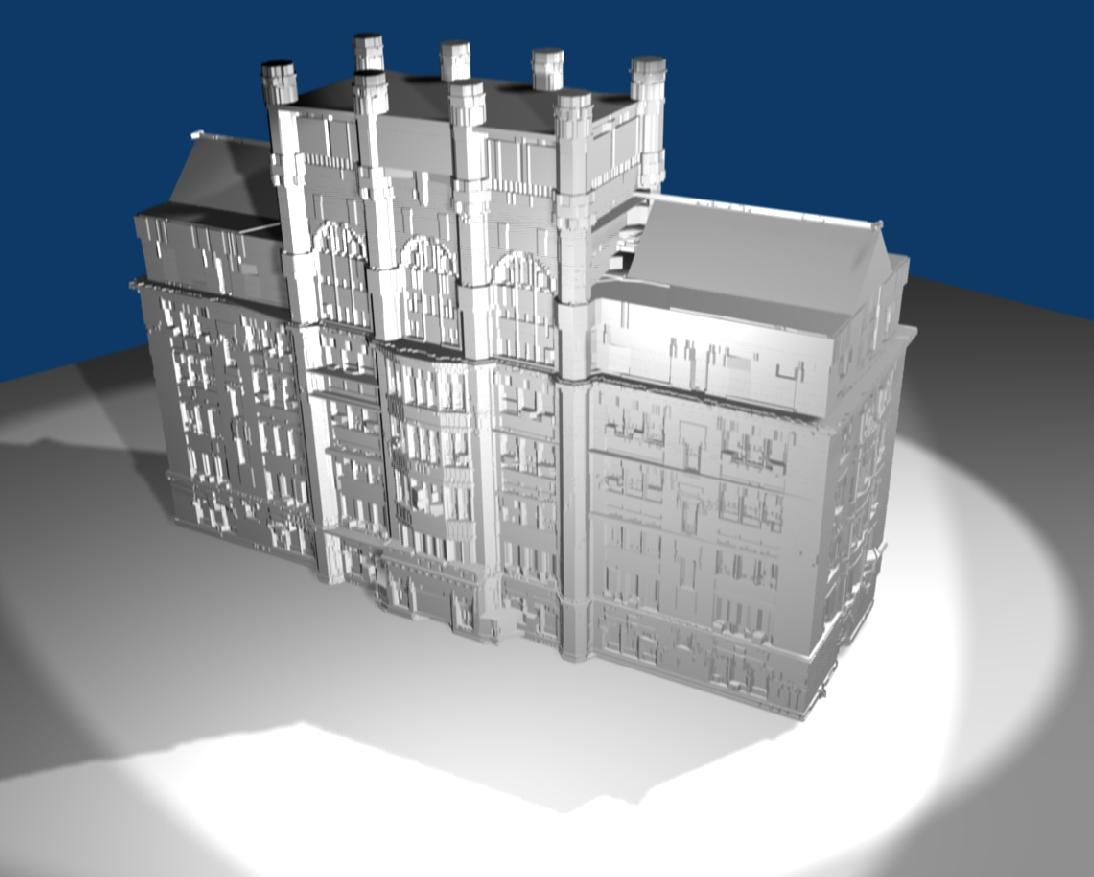
\includegraphics[width=0.8\textwidth]{HunterShaded.jpg} \\
(a) \\
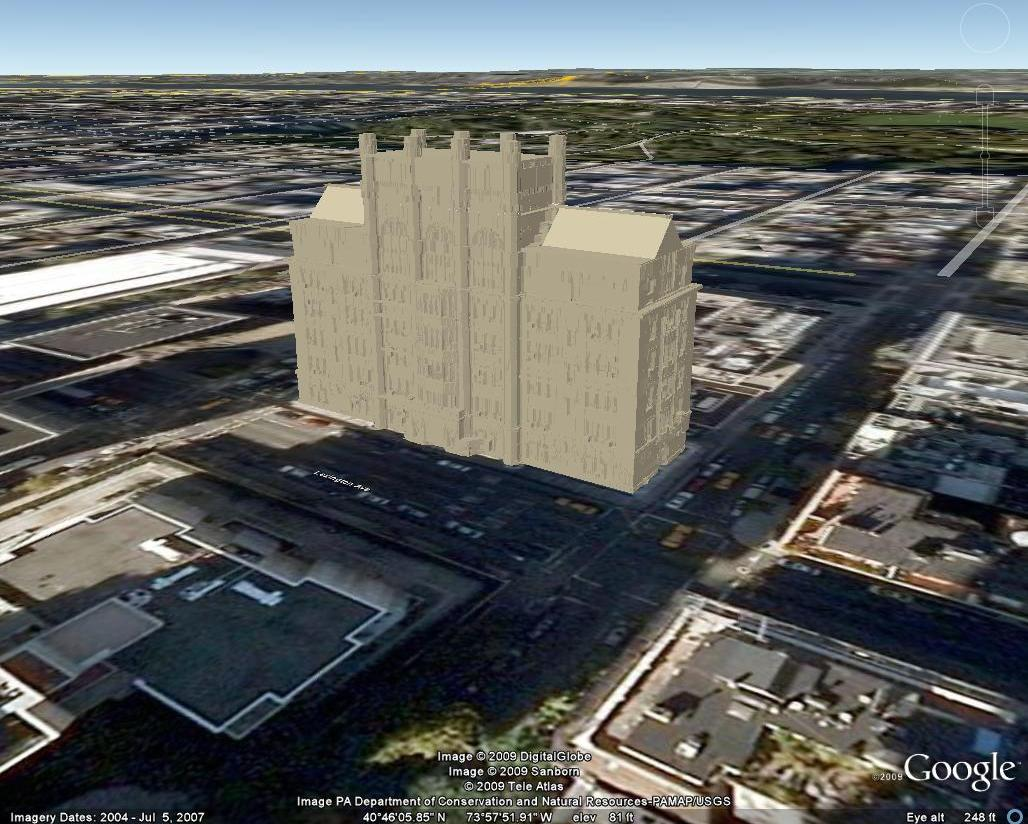
\includegraphics[width=0.8\textwidth]{HunterGE.jpg} \\
(b)
\end{tabular}
\end{center}
\caption{ (a) rendering of lightweight reconstructed model.
(b) The placement of the 3D model on Google Earth.}
\label{fig:OUT}
\end{figure*}

\begin{figure*}[htbp]
\begin{center}
\begin{tabular}{c}
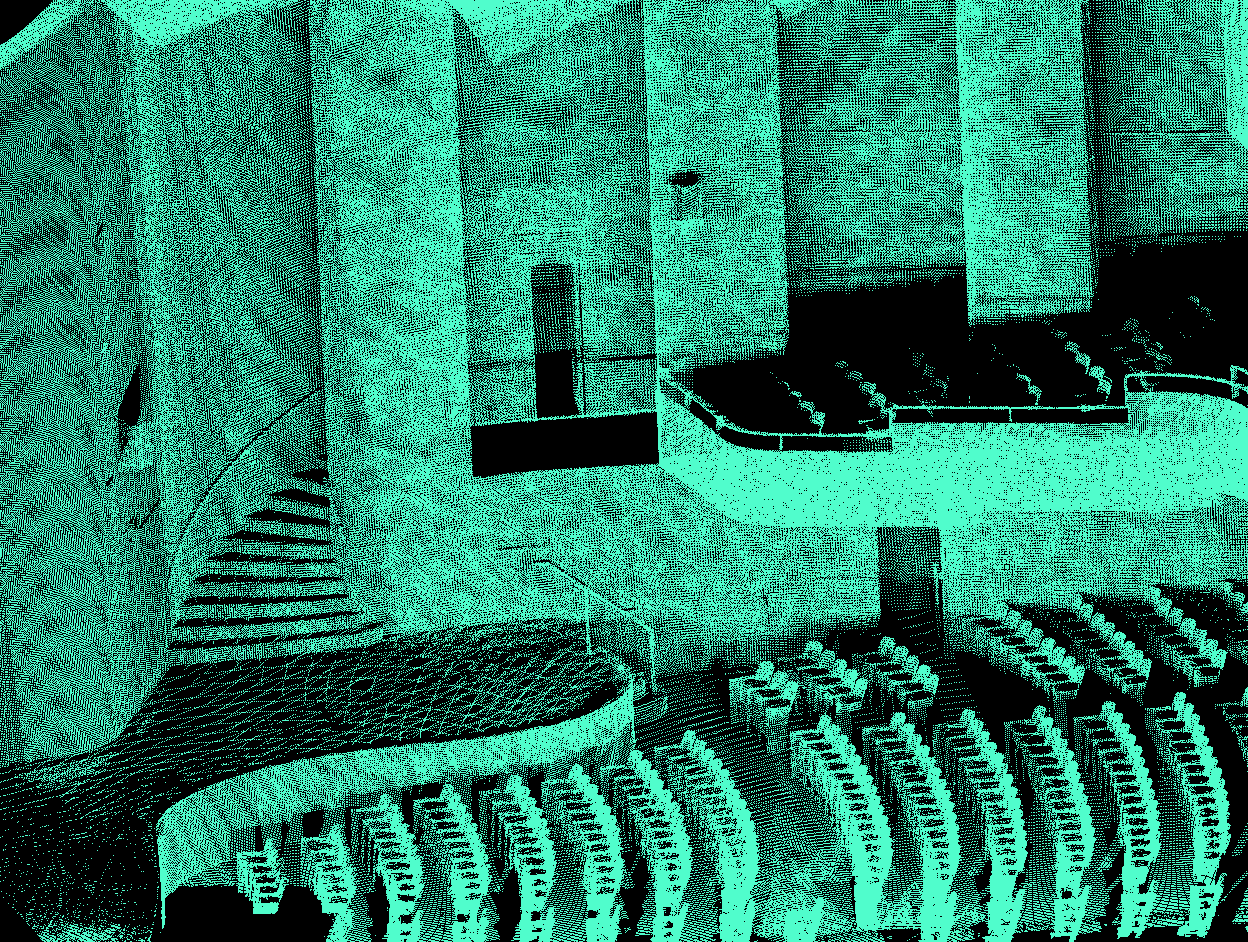
\includegraphics[width=0.8\textwidth]{range_crop.png} \\
(a) \\
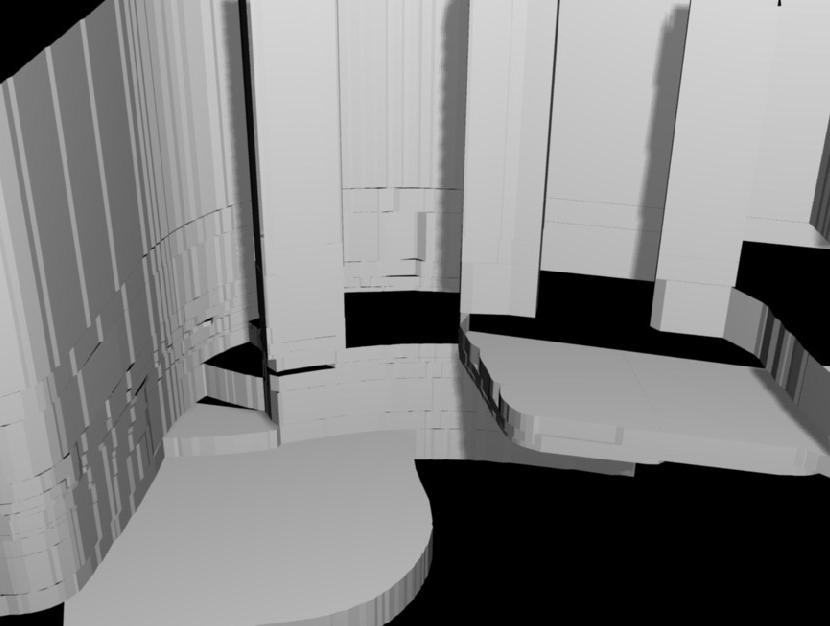
\includegraphics[width=0.8\textwidth]{HunterTheatreShaded.jpg} \\
(b)
\end{tabular}
\end{center}
\caption{The model of an interior scan. (a) Point cloud data and the
(b) reconstructed lightweight 3D model.}
\label{fig:IN}
\end{figure*}

In addition to exterior models, we have also applied the lightweight
reconstruction algorithm to the range data of interior scans.
The snapshot of an interior scan is shown in \Figa{IN}
and its reconstructed 3D model is shown in \Figb{IN}.
This model is primarily reconstructed using the extrusion unit
upon the main structures of the interior.
The chairs and some other fine details were manually culled.
Please note that the model generated in \Figb{IN} is of low resolution.
Any lost detail may be recaptured by using a smaller threshold $\tau_d$
to obtain higher resolution models.

To measure the error of a reconstructed 3D model, we first transform it
to the 3D point cloud coordinate system.
The error $E$ is measured as the distance between the 3D points in the cloud
to their closest planes in the reconstructed model $M$:
\begin{equation}
E = \frac{1}{|X|}\sum_{x\in{X}}{d^2(x, M)}
\label{eq:em}
\end{equation}
where $X$ is the set of 3D points in the point cloud, and distance
$d(x, M) = \text{min}_{p \in M}\lVert x - p \lVert$ is the minimum
Euclidean distance from a 3D point $x$ to its closest face $p$ of $M$.

\begin{figure} [htbp]
\begin{center}
\begin{tabular}{c}
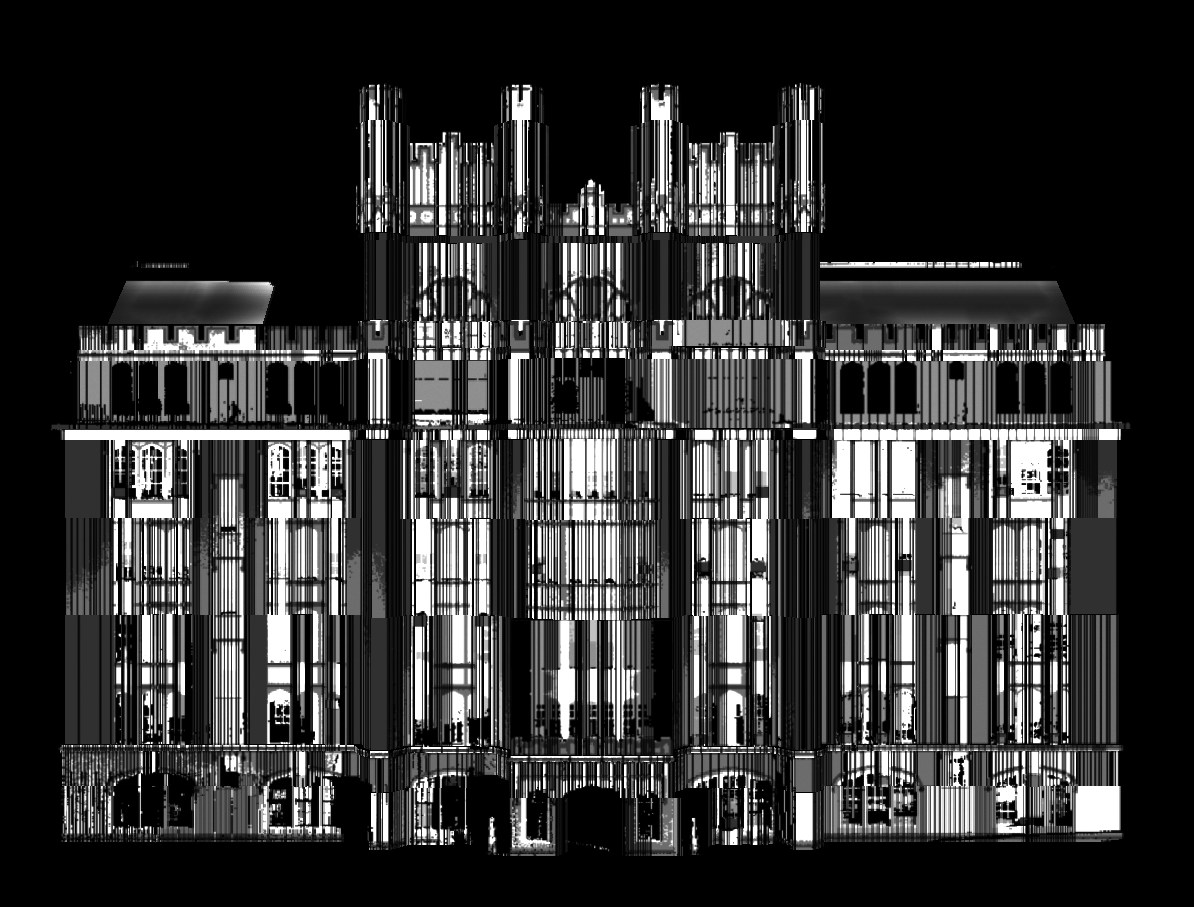
\includegraphics[width=0.8\textwidth]{error_1000_32_4.png} \\
(a) \\
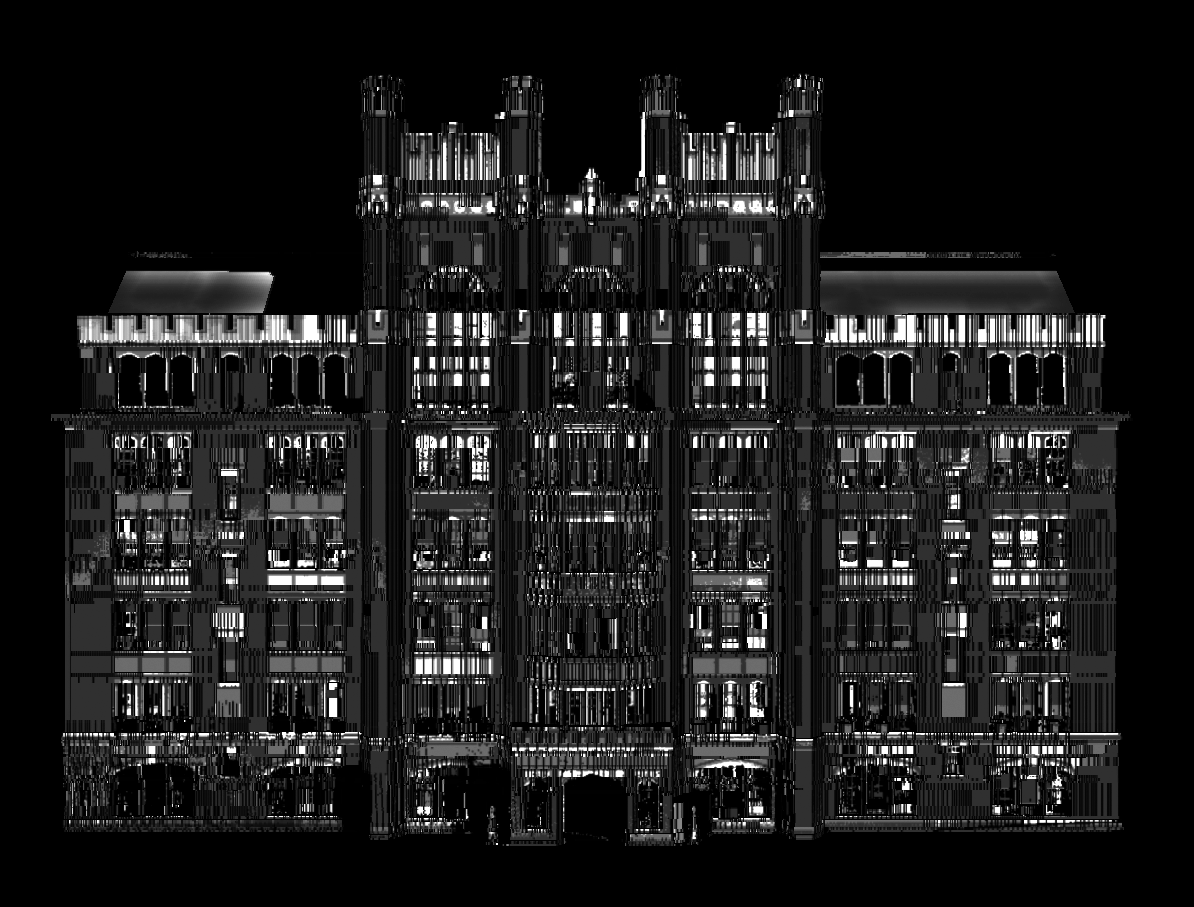
\includegraphics[width=0.8\textwidth]{error_1000_4_1.png} \\
(b)
\end{tabular}
\end{center}
\caption{The deviation map of the 3D point cloud. (a) The result with $\tau_r$ = 4 and $\tau_d$ = 32.
(b) The result with $\tau_r$ = 1 and $\tau_d$ = 4. }
\label{fig:EM}
\end{figure}

To visualize the error between real 3D data and the inferred model,
we generate deviation map images.
Two such images are shown in \Fig{EM} for the point cloud data in
\Figb{IR_2_DXF}.
The deviation maps are constructed as follows.
For each face $p$ of $M$, a corresponding texture image is computed.
The intensity of each pixel in the texture image is determined by the error
of the corresponding 3D points computed by \Eq{em}.
The accuracy of the reconstructed model is controlled by Hausdorff distance
threshold $\tau_d$ and BPA refinement radius $\tau_r$.
Threshold $\tau_d$ determines the accuracy of keyslice detection and $\tau_r$
determines the accuracy of boundary vectorization.

\Tbl{em} lists the relationship among the $\tau_d$, errors,
number of faces, and model size for the input data in \Figb{IR_2_DXF}.
The units for $\tau_d$ and error is in pixels and millimeters, respectively.
The size of the original point cloud for the 3D building is more than 700 MB.
From the table, one can see that even for the most accurate model, the size
is dramatically reduced compared with the original 3D point cloud data.
This is a desirable property for web-based applications (\Figd{IR_2_DXF}).
The low resolution ($\tau_d = 64$) and high resolution ($\tau_d = 4$) models
were generated in 15 and 120 minutes, respectively,
on a laptop PC running an Intel Core 2 T7200 CPU at 2.0 GHz with 2.0 GB RAM.
Future work includes the optimization of the BPA vectorization module since
it consumes approximately 70\% of the computation time.

\setlength{\tabcolsep}{4pt}
\begin{table}[hbtp]
\begin{center}
\begin{tabular}[t]{||c||c|c|c|c||}
\hline
$\tau_{d} $(pixel) & Error (mm)& \# of faces & Size (KB) & time (s) \\ \hline \hline
64 & 0.658 & 1471  & 15  & 1977  (32'57'') \\ \hline 
32 & 0.294 & 3284  & 32  & 2353  (39'13'') \\ \hline
16 & 0.141 & 8574  & 86  & 3008  (50'08'') \\ \hline
8  & 0.131 & 13955 & 137 & 3696  (61'36'') \\ \hline
4  & 0.094 & 27214 & 261 & 5391  (89'51'') \\ \hline
2  & 0.088 & 31331 & 335 & 7586  (126'26'')\\ \hline
1  & 0.083 & 32187 & 337 & 10927 (182'07'')\\ \hline
\end{tabular}
\end{center}
\caption{Error measurements for reconstruction of Thomas Hunter dataset using
Hausdorff distance threshold $\tau_d$ and BPA radius threshold $\tau_r = 4$.}
\label{tbl:em}
\end{table}
\setlength{\tabcolsep}{1.4pt}


\setlength{\tabcolsep}{4pt}
\begin{table}[hbtp]
\begin{center}
\begin{tabular}[t]{||c||c|c|c|c||}
\hline
$\tau_{d} $(pixel) & Error (mm)& \# of faces & Size (KB) & time (s) \\ \hline \hline
64 & 0.085 & 5741   & 55  & 617  (10'17'') \\ \hline
32 & 0.063 & 8614   & 86  & 623  (10'23'') \\ \hline  % key slice 9'
16 & 0.052 & 9810   & 94  & 674  (11'14'') \\ \hline
8  & 0.028 & 15338  & 149 & 740  (12'20'') \\ \hline
4  & 0.022 & 42877  & 420 & 1042 (17'22'') \\ \hline
2  & 0.012 & 91736  & 988 & 1688 (28'08'') \\ \hline % key slice 9'
1  & 0.011 & 101466 & 990 & 1708 (28'28'') \\ \hline
\end{tabular}
\end{center}
\caption{Error measurements for reconstruction of Hunter Theater dataset using
Hausdorff distance threshold $\tau_d$ and BPA radius threshold $\tau_r = 4$.}
\label{tbl:em_theater}
\end{table}
\setlength{\tabcolsep}{1.4pt}

%%%%%%%%%%%%%%%%%%%%%%%%%%%%%%%%
%%%%%%   Model Comparison    %%%
%%%%%%%%%%%%%%%%%%%%%%%%%%%%%%%%
\section{Model Comparison}

Although models generated by 3D BPA are of high resolution, they usually
require excessive storage capacity.
The model in \Fig{TH_BPA}, for example, needs almost 400 MB of storage,
which prevents this solution from being applied to web-based applications.
One way to improve matters is to apply some approximation/decimation
technique to reduce the space required by these models.

The holes in the 3D BPA model in \Fig{TH_BPA} are present in the
original dataset.
They are due to the fact that the laser never reflected back to
the scanner after penetrating the glass windows.
The 3D BPA method is deficient in filling these holes.
We counter this problem by first applying a symmetry-based hole filling
algorithm on the 2D slices to create enhanced slices that are processed
by an adaptive 2D BPA method to fill gaps.
Finally, an extrusion operation is applied to create a watertight 3D model.

\begin{figure}[htbp]
\begin{center}
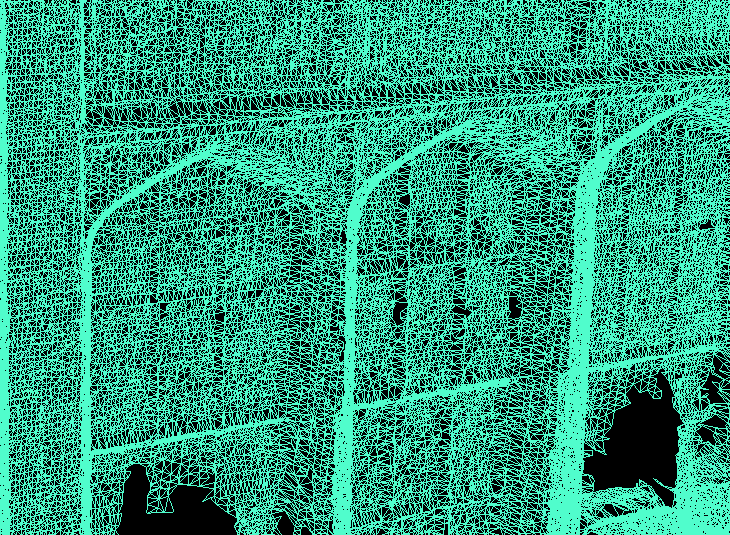
\includegraphics[width=0.8\textwidth]{BPA_TH.png}
\end{center}
\caption{Dense triangulated BPA mesh cropped from \Figb{IR_2_DXF}.}
\label{fig:TH_BPA}
\end{figure}

Among all mesh reduction techniques, {\it qslim} is one of the most
sophisticated and efficient algorithms.
We carried out a comparison between models generated by our proposed
method and those approximated by {\it qslim}.
The comparisons were conducted on models sharing the same number of faces.
It is worth noting that {\it qslim} ran out of memory on the 3D model data
generated by BPA in \Fig{TH_BPA}.
In order to reduce the size of the model for {\it qslim} to work, we had
to either downsample the 3D model generated by BPA or split it into
sub-models which can be handled by {\it qslim}.

\begin{figure}[htbp]
\begin{center}
\begin{tabular}{cc}
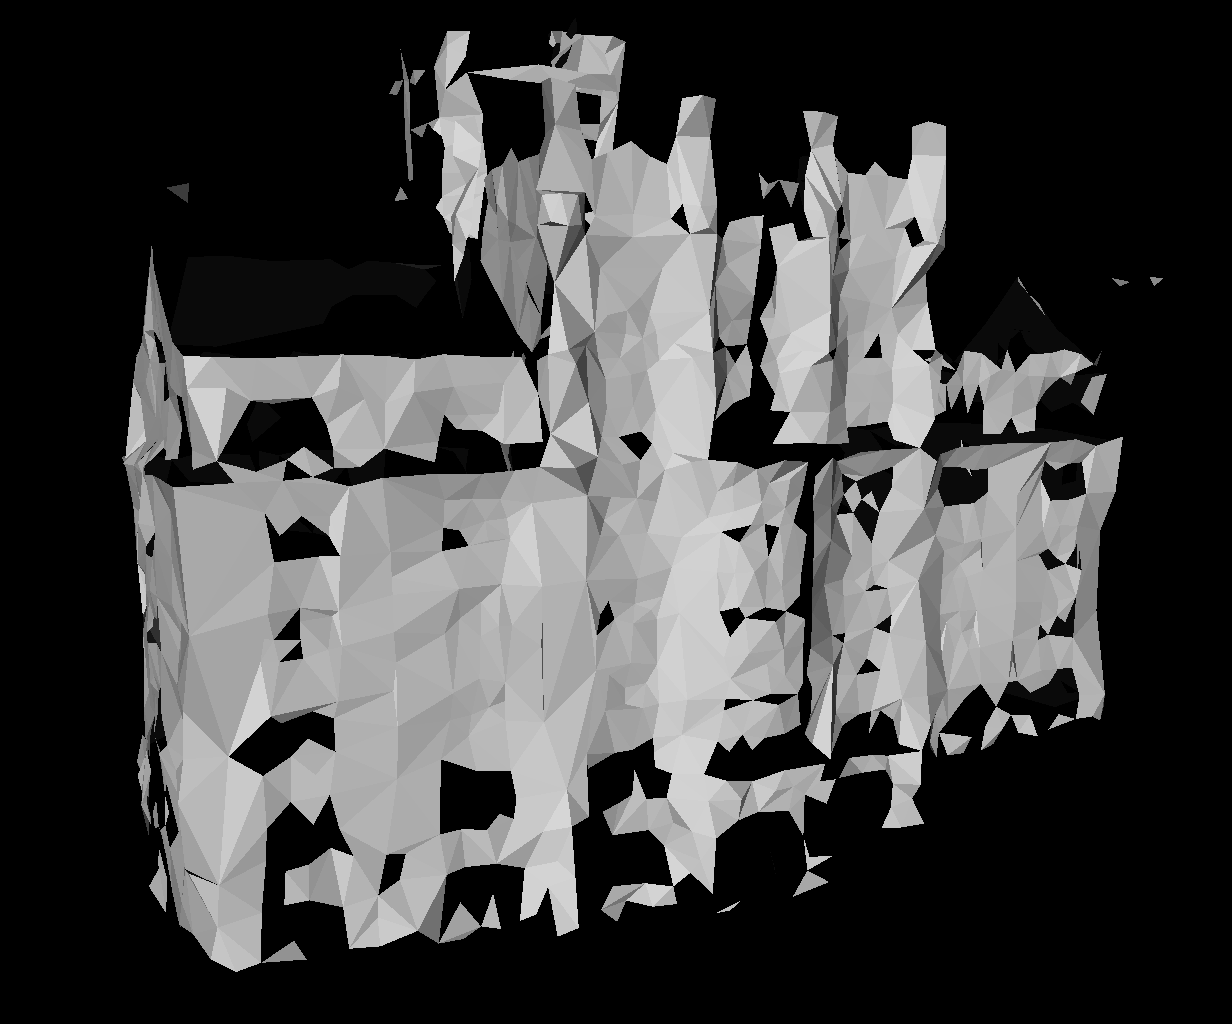
\includegraphics[width=0.45\textwidth]{comp_32_2_qslim.png} &
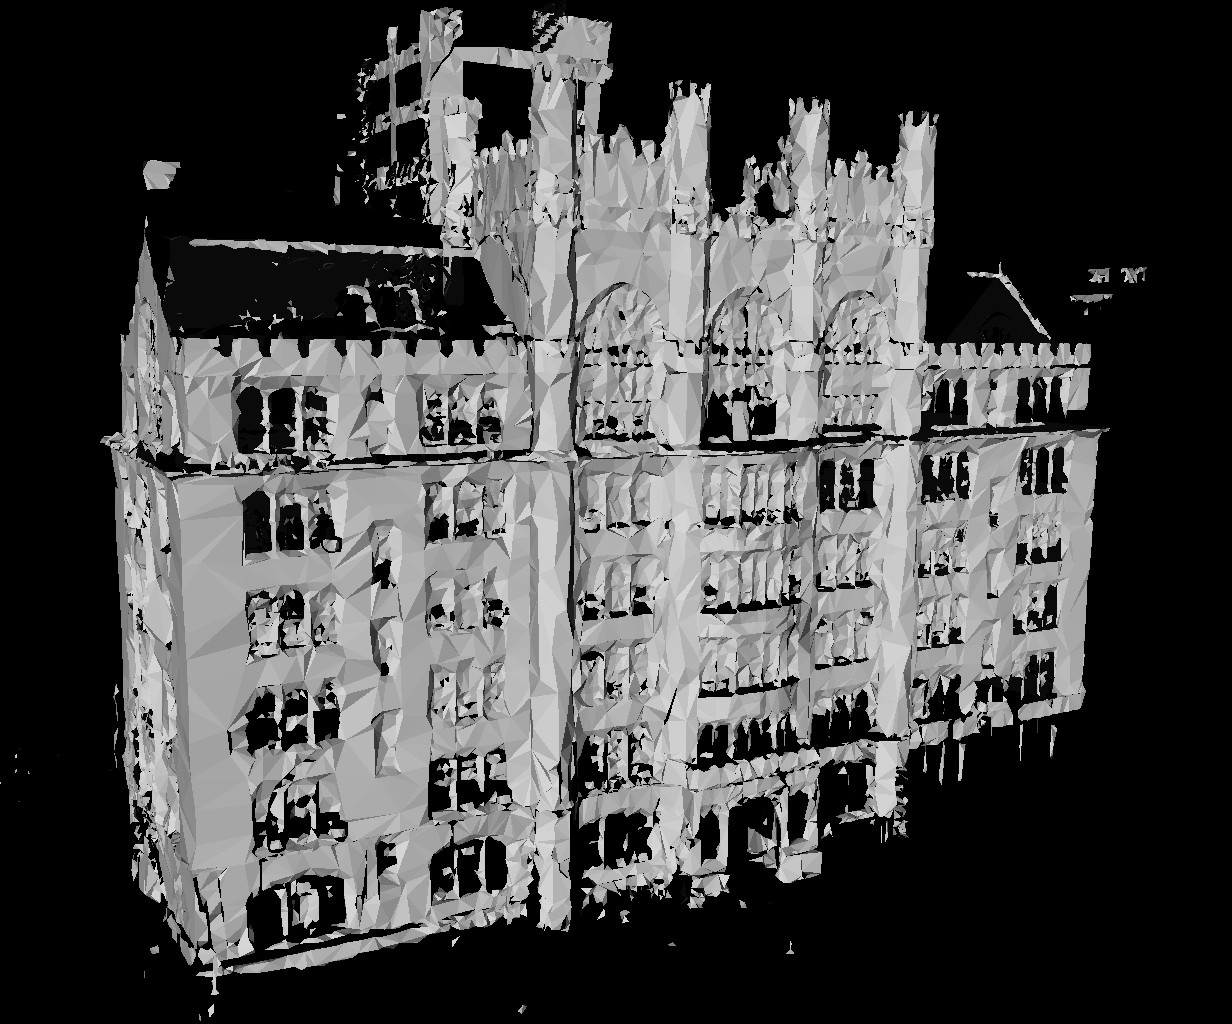
\includegraphics[width=0.45\textwidth]{comp_4_2_qslim.png} \\
(a) & (b) \\
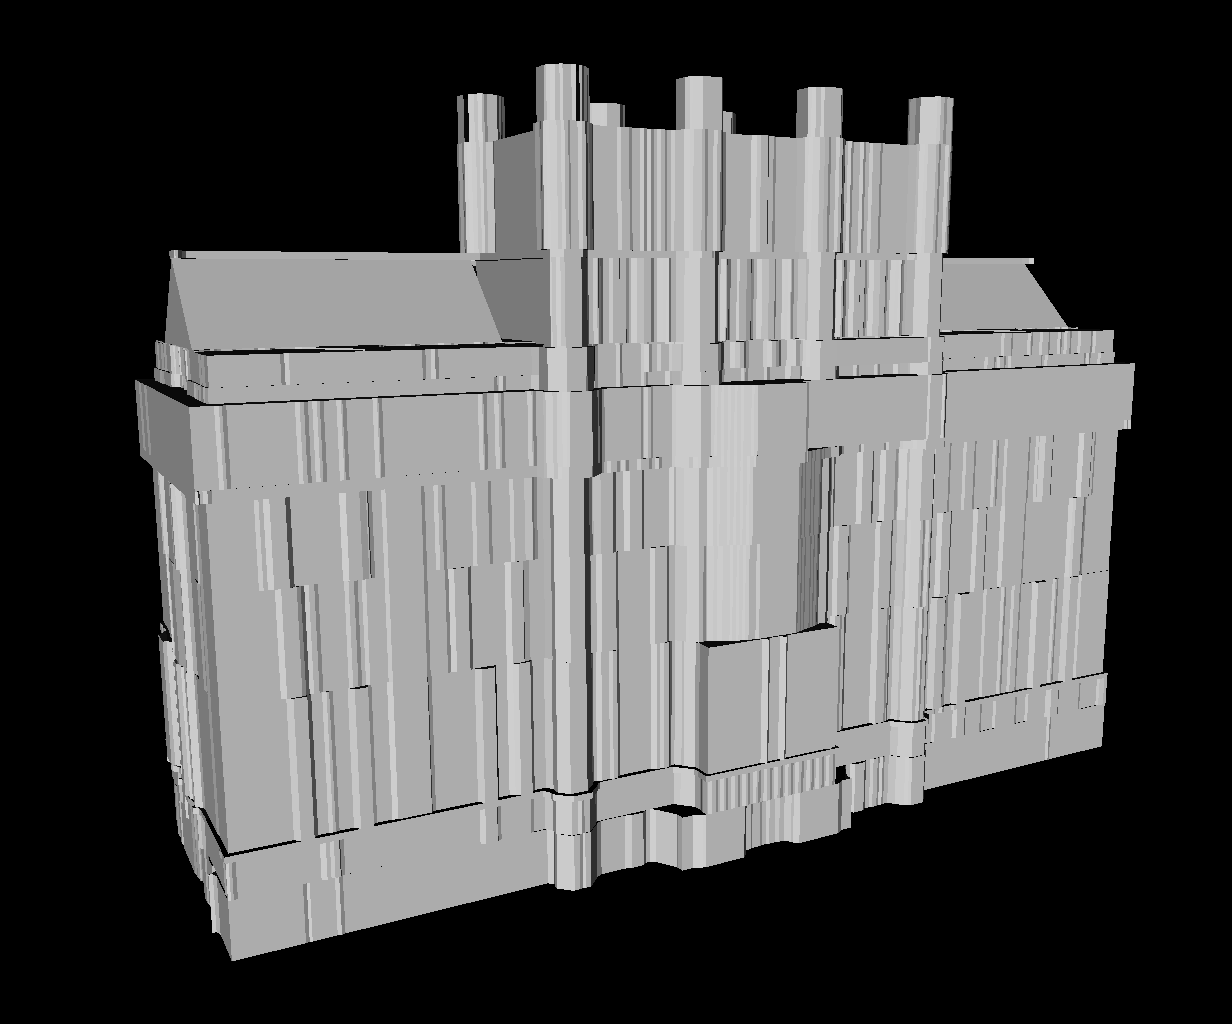
\includegraphics[width=0.45\textwidth]{comp_32_2.png} &
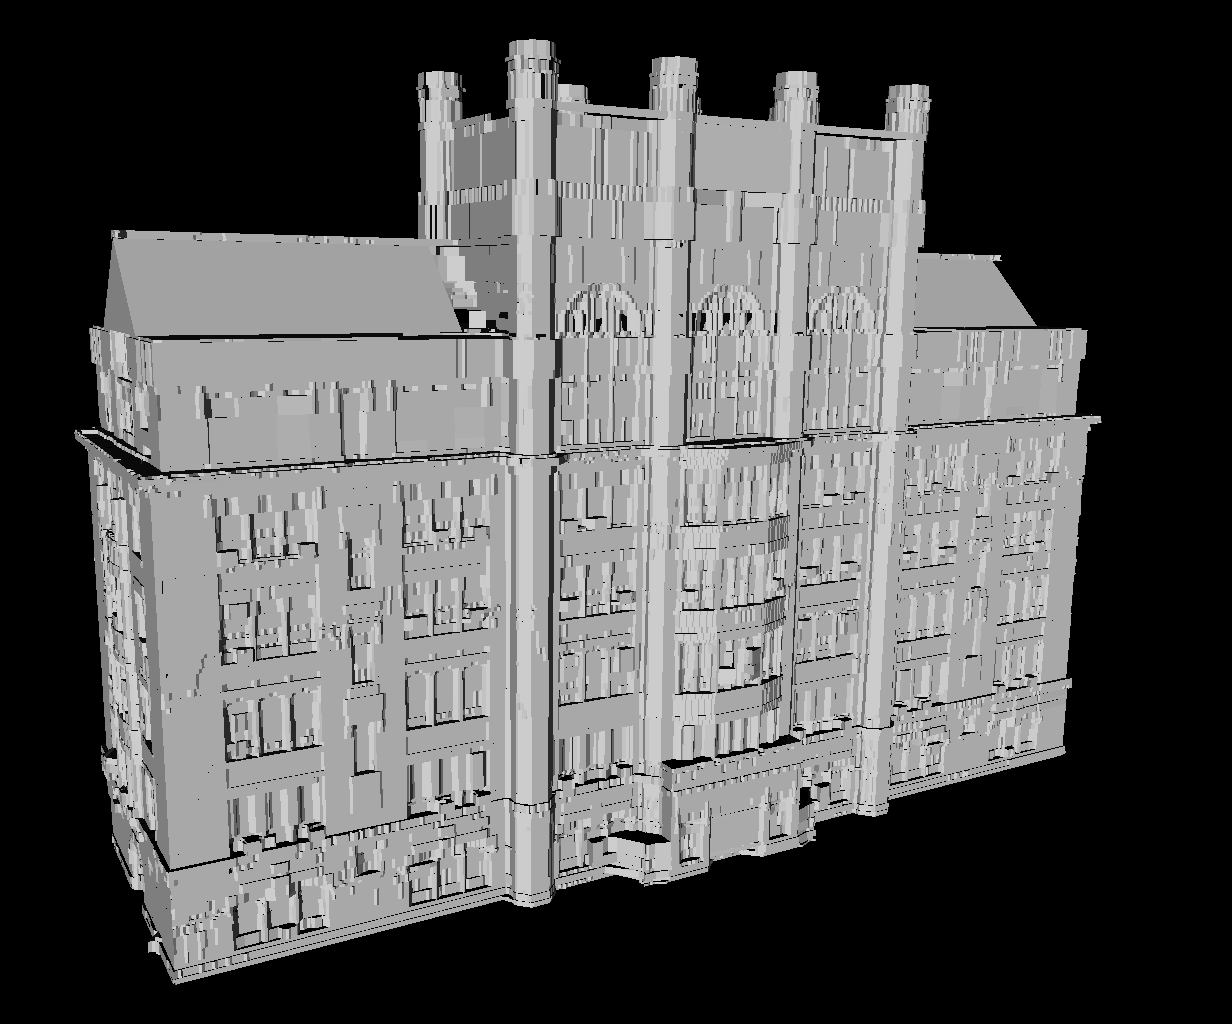
\includegraphics[width=0.45\textwidth]{comp_4_2.png} \\
(c) & (d)
\end{tabular}
\end{center}
\caption{
Models generated by {\it qslim} having (a) 2,000 and (b) 32,000 faces.
Models generated by our approach having (c) 2,000 and (d) 32,000 faces.}
\label{fig:TH_comp}
\end{figure}

\Figa{TH_comp} and \Figc{TH_comp} respectively depict the models generated
by {\it qslim} and our proposed method with approximately 2,000 faces each.
Higher resolution models with roughly 32,000 faces each are shown in
\Figb{TH_comp} and \Figd{TH_comp}.
Notice that the models approximated by {\it qslim} are inferior since they
do not preserve the sharpness of the original model and are replete with
holes. Our symmetry detector and extrusion operation guarantees no holes.

